\section{Privacy Via {\methodName}}
In this section we describe our algorithm, {\methodName}, which injects uncertainty to the given uncertain graph so that it becomes {\keobf} while preserving as much the stochastic nature as possible. A key feature of our method is to seamlessly integrate edge uncertainty and possible world semantics into the core of anonymization operators. 
% 
\subsection{Heuristic for Edge Perturbation}

% It is non-trivial to figure out the optimal set of edges that balances privacy gain and structural distortion. 
Selecting the set of edges subject to modification which balances privacy gain and structural distortion is 
a key component of graph anonymization. 
It involves consideration over the exponential number of edge combinations. 
Recently, the most popular paradigm for solving such problems has been using a class of heuristics. 
Successes of this approach include
(1) anonymity-aware ones that suggest injecting more considerable noise to unique nodes~\cite{Ying2009,Boldi_Injecting_2012,Hay_Anonymizing_2007} 
(2) utility-aware ones that indicate avoiding distortion over “bridge” edges whose deletion/addition would significantly impact the graph structure~\cite{Wang2011,Ninggal_Utility_2015}. 
The judicious edge selection must involve two types of heuristics which complement each other. 
Individually, they are far less effective. 
Nevertheless, they have not been explored yet in the context of uncertain graphs.

Motived by the above, we first generalize the calibration of uniqueness via the use of KL-divergence. 
Second, we propose a generalized edge relevance criterion from an information-theoretic perspective.
Besides, we develop an efficient algorithm for its computation in the context of uncertain graphs.
And, we show the use of such a criterion boosts XXX efficiently and straightforwardly.

\subsubsection{Generalized Uniqueness}

\begin{figure}
	\centering
        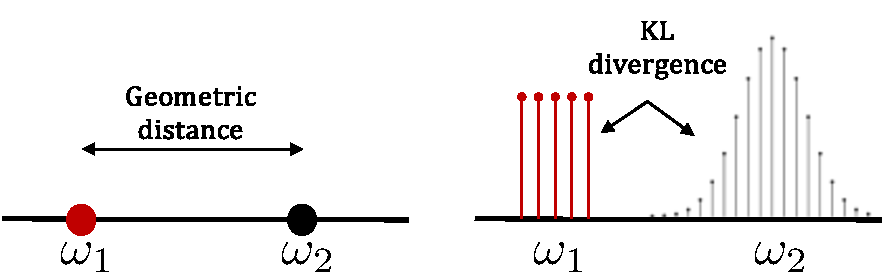
\includegraphics[width=\linewidth]{ill/shift_distance.pdf}
    \caption{Deterministic values and stochastic values.}
\end{figure}
The uniqueness criterion was used to measure how unique a given node is among all the nodes in the graph w.r.t a specific property. 
For a given node, its uniqueness score is the inverse of the commonness score of its property value $w$.
While, the commonness score of $w$ amounts to the weighted average distance among all other property values. 

The conventional method merely formulates node properties as discrete values and relies on the geometric distance function to measure their distance.  
Thus, it fails to handle our problem where the property values are stochastic.   
In this work, we extend the preliminary version for handing the stochastic case. 
We consider the use of probability distributions, which are essential characteristics of uncertain property values, in the measuring similarity between uncertain property values. 
We systematically model uncertain property values in both continuous and discrete domains as continuous and discrete random variables, respectively.
We use the well known Kullback-Leibler divergence to measure the distance between random variables with parameterized distributions. 
The generalized version of uniqueness score can then be formalized as
\begin{definition}
    \textbf{Uniqueness Score}
     Let $P:V \rightarrow  \Omega_{P}$ be a property on the set of nodes $V$ of the uncertain graph, 
     let $d$ be a KL divergence function, and let $\theta >0$  be a parameter. 
  	 Then the $\theta-$commonness of the property values $\omega$
  	 is $C_{\theta}(\omega):= \sum_{u \in V} \Phi_{0,\theta}(KL(\omega, P(v)))$,   
	 while the corresponding uniqueness is $U_{\theta}:= \frac{1}{C_{\theta}(\omega)}$. 
	 \vspace{-2pt}
\end{definition} 
Note that, the weights decays exponentially as a function of the KL divergence, 
and the parameter $\theta$ determines the decay rate. 
We set $\theta=\sigma$ as the injected noise blurs the meta distribution of property values. 
 
\subsubsection{Generalized Edge Relevance}

It is clear that alteration over a single edge would produce local structural change and send ripples through the rest of the graph. 
The incurred structural distortion varies on the topological role of the edge subjecting to alteration, even with the same amount of alteration. 
% Observe that edges with different roles will incur significantly different structural changes even with the same amount of injected noise. 
Targets at the high utility, we should penalize modification over structurally critical edges.  
Thus, we need measure the edge relevance w.r.t graph structure. 

There are many potential ways to measure it. 
Importantly, the metric must be fitted to the context of uncertain graphs.
Inspired by the concept of cut-edge, we measure the edge relevance of a given edge $e$
as the amount of structural distortion, measured by reliability discrepancy, caused by the unit noise subjects to the edge $e$, as follow. 
\begin{equation*}
    \mathcal{ERR}({e}) = \lim_{r_{e} \rightarrow 0} \frac{\Delta(\mathcal{G}+r_{e})}{r_{e}} 
                      = \sum_{u,v} \frac{|R_{u,v}(\mathcal{G}+r_{e}) -R_{u,v}(\mathcal{G})|} {r_{e}}
\end{equation*}

In deterministic graphs, a cut-edge of a graph is an edge whose deletion increases the number of connected components. 
In probabilistic graphs, $\mathcal{ERR}$ is used to generalize this concept by quantifying the stochastic impact of adding/deleting edge partially over the connectivity of all the possible worlds.
while the cut-edge is a binary classification, the $ERR$ value lies in the continuous range, and quantify the probability if the connected pairs holds in a possible world. 

In order to explore this point further, we have illustrate a probabilistic graph in Figure~\ref{}. 

% switch into the lemma format 
% The factorization lemma~\cite{Jin_Distance_2011} indicates
% \begin{align*}
%     R_{u,v}(\mathcal{G}+r_{e}) -R_{u,v}(\mathcal{G}) = r_{e} \cdot \big[ R_{u,v}(\mathcal{G}_{e})-R_{u,v}(\mathcal{G}_{\hat{e}}) \big]
% \end{align*}
% Then, the edge relevance $\mathcal{ERR}$ can then formulate as
% \begin{equation*}
%     \mathcal{ERR}(e) = \sum_{u,v} R_{u,v}(\mathcal{G}_{e}) \big- \sum_{u,v} R_{u,v}(\mathcal{G}_{\bar{e}})
% \end{equation*}

Observe that, $\mathcal{ERR}(e)$ amounts to the number difference of connected node pairs between two neighbor uncertain graphs $\mathcal{G}_{e}$ and $\mathcal{G}_{\bar{e}}$, 
where $\mathcal{G}_{e}$ and $\mathcal{G}_{\bar{e}}$ are identical to $\mathcal{G}$ with the exception that $p(e)=1$ in the former and $p(e)=0$ in the later. 





% We also show its computation can be achieved via Monte-Carlo sampling with an acceptable time complexity $\mathcal{O} (N \cdot T)$, where $N$ is the number of samples and $T$ is time complexity for the employed connected component detection algorithm.~\footnote{ The union-and-find method is used in this work.} The key idea is to memorize the calculated result (\# of connected node pairs) over samples. For each edge $e$, we group then aggregate results of samples according to edge existence. And, the vertex reliability relevance $\mathcal{VRR}$ amounts to the weighted sum of $\mathcal{ERR}$ values.











